%%%%%%%%%%%%%%%%%% CALCULUS ON MANIFOLDS

\chapter{Calculus on Manifolds}

\section{What is a Manifold?}

A $m$-dimensional {\sc Manifold} is a (topological) space which at each point looks locally like $\R^m$. Note that $m$ is a fixed number, and defines the dimension of the manifold.

\begin{Def}[Manifold]
  A {\sc Manifold}, $M$, is a topological space homeomorphic to $\R^m$.
\end{Def}



Examples of manifolds are  the body of a cylinder,  the spheres ($S^m$), the torus ($T^m$).

%% \begin{center}
%%   \begin{tikzpicture}[baseline]
%%     \begin{axis}[hide axis,axis equal=true,]
%%     \addplot3[  
%%       surf, shader=interp,
%%       unit vector ratio=1 1 1,
%%       colormap/greenyellow,
%%       %mesh,
%%       fill=white,      
%%       point meta=x,
%%       samples=20,
%%       samples y=40,
%%       domain=0:180,
%%       y domain=0:360,
%%     ] (                                                                         
%%              {sin(x)*cos(y)},                                                   
%%              {sin(x)*sin(y)},                                                   
%%              {cos(x)}                                                           
%%    );          
%%     \end{axis}
%%   \end{tikzpicture}
%%   \hspace{1cm}
%%   \begin{tikzpicture}[baseline]
%%     \begin{axis}
%%       [
%%         hide axis,
%%         %view={60}{30},
%%         axis equal image,
%%       ]
%%       \addplot3 [
%%         surf, shader=interp,
%%         point meta=x,
%%         colormap/greenyellow,
%%         samples=40,
%%         samples y=20,
%%         z buffer=sort,
%%         domain=0:360,
%%         y domain=0:360
%%       ] (
%%                 {(3.5 + 0.5*cos(y))*cos(x)},
%%                 {(3.5 + 0.5*cos(y))*sin(x)},
%%                 {0.5*sin(y)});
%%       \addplot3 [
%%         samples=40,
%%         samples y=1,
%%         domain=0:360,
%%         thick
%%       ] (
%%                 {(3.5 + 0.5*cos(80))*cos(x)},
%%                 {(3.5 + 0.5*cos(80))*sin(x)},
%%                 {0.5*sin(80)});
%%     \addplot3 [
%%       samples=10,
%%       samples y=1,
%%       domain=-65:130,
%%       thick
%%     ] (
%%               {3.5 + 0.5*cos(x)},
%%               {0},
%%               {0.5*sin(x)});
%%     \end{axis}
%%   \end{tikzpicture}
%% \end{center}
\begin{center}
  \begin{tabular}{cc}
    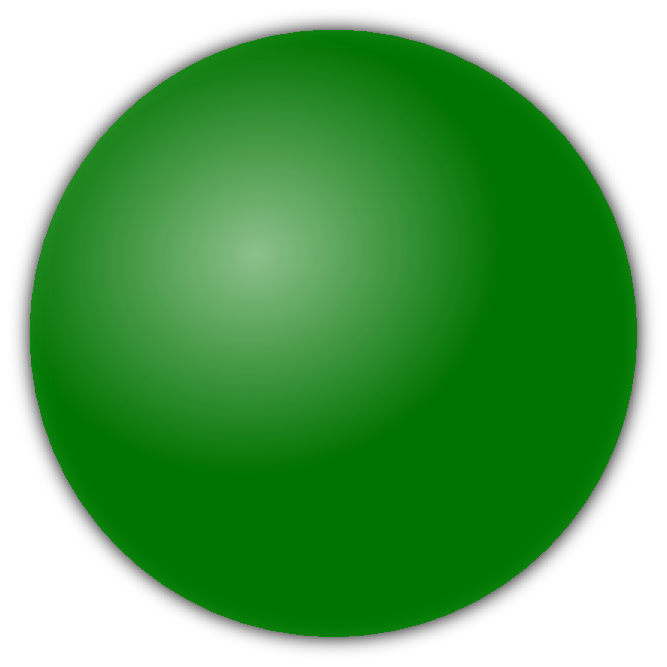
\includegraphics[scale=.4]{Pict/Sphere.pdf}  & 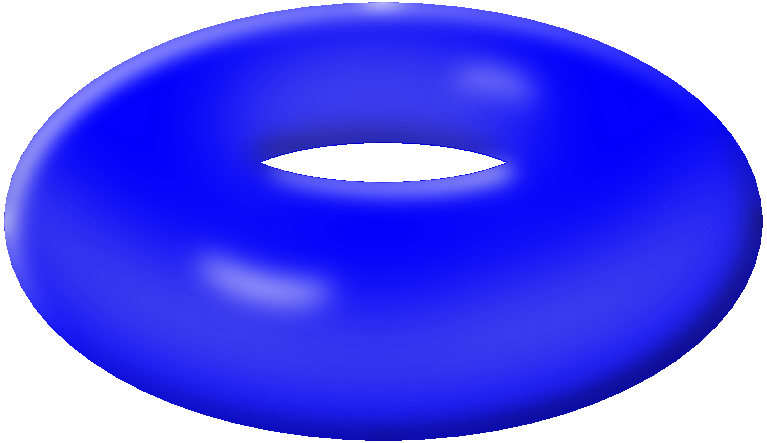
\includegraphics[scale=.4]{Pict/Torus.pdf}
  \end{tabular}
\end{center}
%% \begin{figure}[H]
%%   \begin{center}
%%      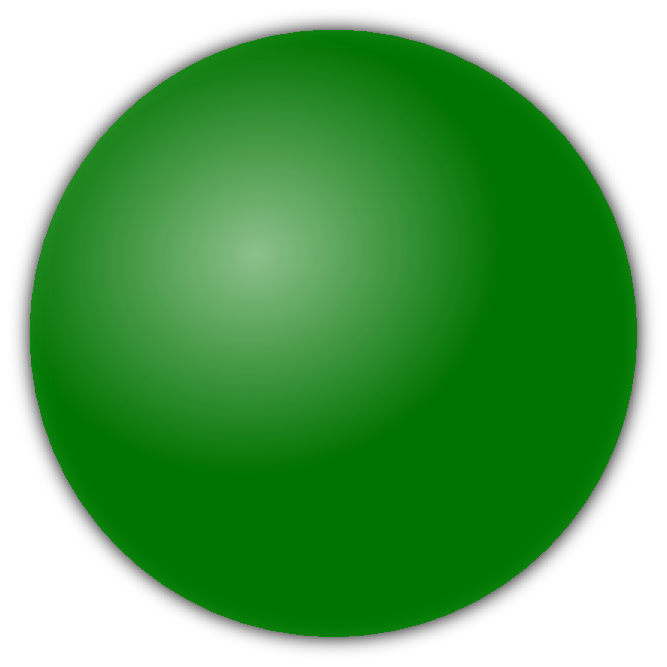
\includegraphics[scale=.4]{Pict/Sphere.pdf} 
%%      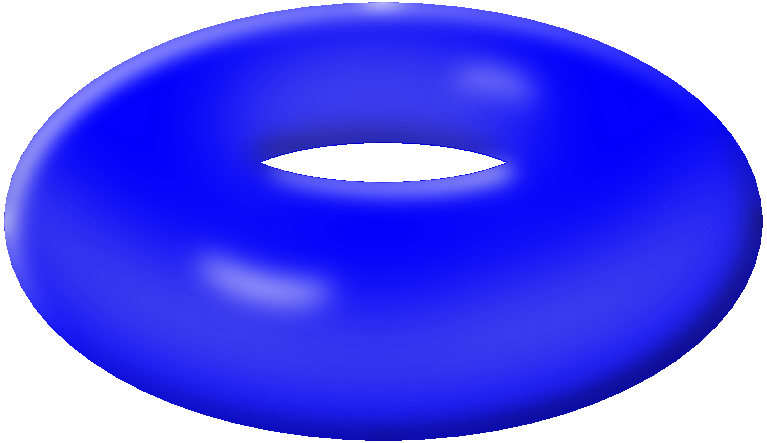
\includegraphics[scale=.4]{Pict/Torus.pdf}
%%   \end{center}
%%   \caption{Examples of manifolds}
%% \end{figure}


More illustrative is an example of a non-manifold, such as the body of a cone. A cone is not a manifold because the neighbourhood of the apex looks not line $\R^2$.
\begin{center}
  \begin{tikzpicture}[scale=1.5,
      spy using outlines={circle, magnification=6, size=2.5cm,connect spies}] 

    \pgfmathsetmacro{\a}{3}
    \pgfmathsetmacro{\b}{5}
    \pgfmathsetmacro{\th}{30}
    \pgfmathsetmacro{\ph}{atan(\a * tan(\th) / \b)}
    \pgfmathsetmacro{\r}{\a * tan(\th)}
    \pgfmathsetmacro{\h}{sqrt(\a*\a +\r*\r)}
    \pgfmathsetmacro{\H}{sqrt(\b*\b +\r*\r)}

    \coordinate (O) at (0,0);
    \coordinate (X) at (0,{\b-\a});

    \draw[thick,dashed] (X)  +(270+\th:\h) arc (90-\ph:90+\ph:\H);
    \shadedraw[left color=blue, right color= blue!60!black, middle color=blue!60!white, shading angle={90-\th}, opacity=.7] (X) -- +(270-\th:\h) arc (270-\ph:270+\ph:\H) --cycle;
    

    \spy on (X) in node at (5,1);
  \end{tikzpicture}
\end{center}

\section{Geometrical Objects on Manifolds}

One knows how to define 

\subsection{Vectors}

\subsection{One-Forms}

\subsection{Tensors}

\begin{Ebox}
  How do the components of $T$ transform? Where 
  \begin{align}
    T= T^{a_1\cdots a_p}{}_{b_1\cdots b_q} \partial_{a_1}\otimes\partial_{a_p}\otimes dx^{b_1}\otimes dx^{b_q}.
  \end{align}
\end{Ebox}

\section{Induced Maps and Submanifolds}

\subsection{Differential Map}

\subsection{Pullback Map}

\begin{Ebox}
  Let $M$, $N$ and $P$ be manifolds, and $ f:M\to N$, $g:N\to P$,  be maps between manifolds. 

  Show
  \begin{align*}
    (g\circ f)_* &= g_*\circ f_*\\
    (g\circ f)^* &= g^*\circ f^*
  \end{align*}
\end{Ebox}

\subsection{Submanifolds}

\section{Flows and Lie Derivative}

\begin{Ebox}
  For the example with $X=x\partial_y -y\partial_x$, show explicitly that 
  \begin{align}
    \sigma_t\circ \sigma_s = \sigma_{t+s}.
  \end{align}
\end{Ebox}


\begin{Ebox}
  Find the flow generated by
  \begin{align}
    X = x\partial_y +y\partial_x.
  \end{align}
\end{Ebox}

\begin{Ebox}
  \begin{itemize}
  \item Let $X$ and $Y$ be vector fields on $M$ and $f:M\to\R$ a function.
    \begin{itemize}
    \item Calculate $\Li_{X}f$.
    \item Calculate $\Li_{fX}Y$.
    \item Calculate $\Li_{X}fY$.
    \end{itemize}
  \item  Let $X$ and $Y$ be vector fields on $M$ and $f:M\to N$ a map between manifolds. Show that
    \begin{align}
      f_*\comm{X}{Y} =\comm{f_*X}{f_*Y}.
    \end{align}
  \item Let $\omega\in\Lambda^1(M)$ be a one-form on $M$. Calculate
    \begin{align}
      \Li_X \omega
    \end{align}
  \end{itemize}
\end{Ebox}
